%% ProcessMusic.tex
%% V0.1
%% 2012/10/23
%% by Kyle Kastner
%%
%% requires IEEEtran.cls version 1.7 or later
%% This file based on content from http://www.ctan.org/tex-archive/macros/latex/contrib/IEEEtran/

\documentclass[journal]{IEEEtran}
\usepackage[labelfont=bf]{caption}
\captionsetup[figure]{labelformat=parens}
\usepackage{graphicx}
\usepackage{amsmath}
\usepackage{flushend}
\newcommand\numberthis{\addtocounter{equation}{1}\tag{\theequation}}
\begin{document}
\title{Probabilistic Matrix Factorization Methods}

\author{Kyle Kastner\\University of Texas-San Antonio}

\maketitle

\begin{abstract}
Probabilistic matrix factorization is a recent development in the field of sparse matrix factorization methods, developed partially to address issues
in modern recommender systems. Kernelized probabilistic matrix factorization offers tuneable model extensions to the probabilistic matrix
factorization framework, allowing for models which incorporate prior information about the connections between available measurements.
\end{abstract}
% IEEEtran.cls defaults to using nonbold math in the Abstract.
% This preserves the distinction between vectors and scalars. However,
% if the journal you are submitting to favors bold math in the abstract,
% then you can use LaTeX's standard command \boldmath at the very start
% of the abstract to achieve this. Many IEEE journals frown on math
% in the abstract anyway.

% Note that keywords are not normally used for peerreview papers.
\begin{IEEEkeywords}
Matrix factorization, adjacency graph, matrix kernel, recommender systems, prediction, machine learning 
\end{IEEEkeywords}

\IEEEpeerreviewmaketitle
\section{Introduction}
\IEEEPARstart{M}{atrix} factorization methods have recently gained attention in the machine learning community, due to their unique advantages sparse 
matrix recommender systems. These innovations have been fueled, at least in part, by the growing needs of social networks and online content providers to
provide customized product recommendations on a per user basis. By taking a sparse matrix \begin{math}A\end{math} as input, and attempting to 
factorize the measured values into "factors" which describe attributes of each row, \begin{math}U\end{math}, and factors of each 
column, \begin{math}V\end{math}, it is possible to estimate a value for an 
unmeasured matrix entry \begin{math}A_{i,j}\end{math} by taking the vector product of the corresponding entries \begin{math} U_i V_j^T
\end{math}. 

This paper will discuss three methods of performing this matrix decomposition: singular value decomposition (SVD), 
probabilistic matrix factorization (PMF), and kernelized probabilistic matrix factorization (KPMF). Implementation details and comparisons between
the three methods will also be discussed.

\section{Testing Data}
For evaluating the performance of each of these algorithms, the classic Lena image was used. This image was then converted into a sparse matrix via 
rejection sampling. For testing, sparseness \begin{math}s = .75\end{math} was chosen. Though these algorithms are not specifically designed to operate on 
images, this format is very convenient for qualitative inspection of algorithmic performance. Root mean square error (RMSE, Eq. \ref{eq:RMSE}) 
is also used as a quantitative comparison metric.
\begin{equation}
    RMSE=\sqrt{\frac{\sum\limits^N_{n=1}(x_n-\tilde{x}_{n})^2}{N}}
\label{eq:RMSE}
\end{equation}
A visual representation of the tesing data can be seen in Fig. \ref{fig:lena} and \ref{fig:sparselena}.
\begin{figure}[h!]
\centering
    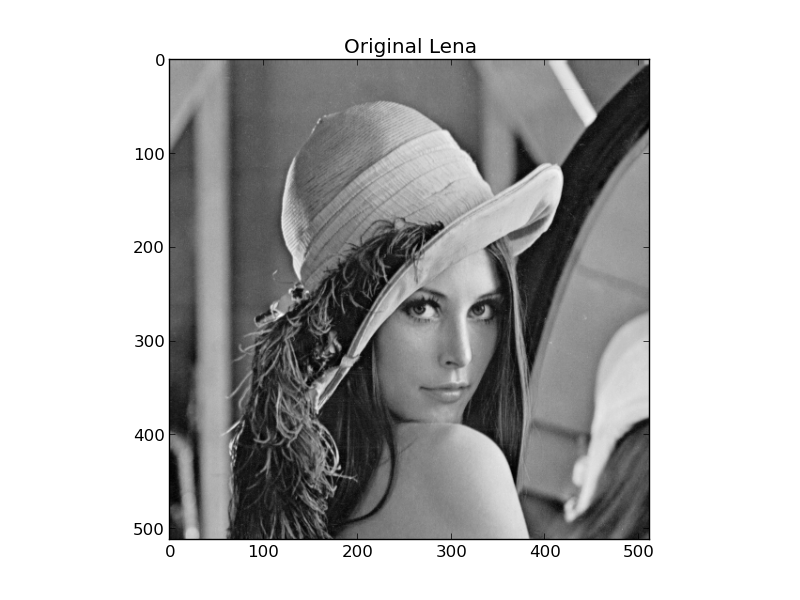
\includegraphics[width=0.45\textwidth]{lena.png}
    \caption{Full matrix Lena image data}
    \label{fig:lena}
\end{figure}
\begin{figure}[h!]
\centering
    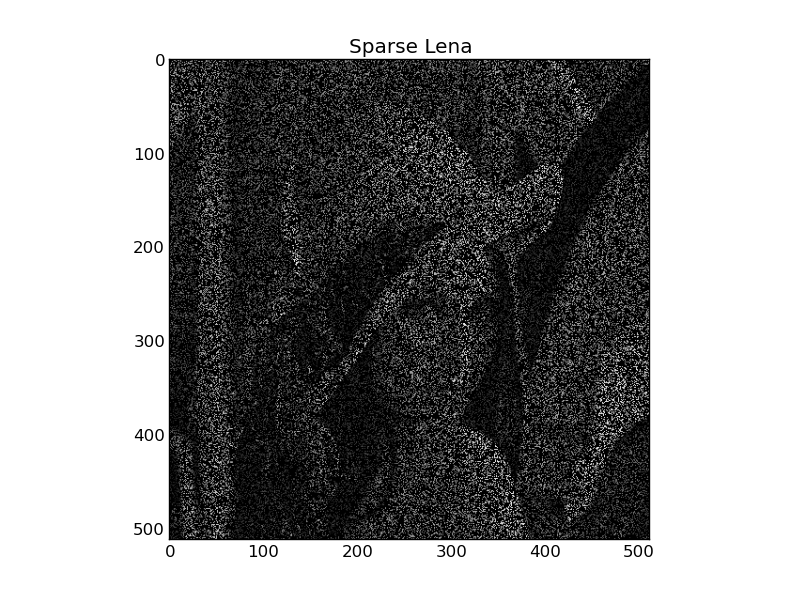
\includegraphics[width=0.45\textwidth]{sparselena.png}
    \caption{Sparse matrix Lena image data}
    \label{fig:sparselena}
\end{figure}
\section{SVD}
The SVD is a very well known technique in linear algebra, statistics, and signal processing. The SVD is based on eigendecomposition, and is often used 
in a similar manner as principal component analysis (PCA) and linear discriminant analysis (LDA), in order to decompose a matrix into 
orthogonal basis vectors that describe the row and column components. The goal of SVD is to find a solution to Eq. \ref{eq:SVD}.
\begin{equation}
    A=U \Sigma V^T
\label{eq:SVD}
\end{equation}
There are many formulas for the numerical calculation of the SVD, though one of the most common methods used is the Lanczos
algorithm. The reference implementation for this paper used Python, with the scipy and numpy libraries. These Python libraries in turn used 
the ARPACK FORTRAN library, which implements the Lanczos algorithm in order to perform the SVD computation. The SVD was originally
developed for full-matrix decomposition, but it also functions for sparse matrices. The resultant matrices \begin{math}U,V\end{math} are of
dimension \begin{math}N \times K\end{math} and \begin{math}K \times N\end{math} respectively, where the number of support parameters
\begin{math}K\end{math} allows for a tradeoff between computational complexity and reconstruction quality. All computations in this experiment used
\begin{math}K=10\end{math} for the number of factors per row and column element. 
\begin{figure}[h!]
\centering
    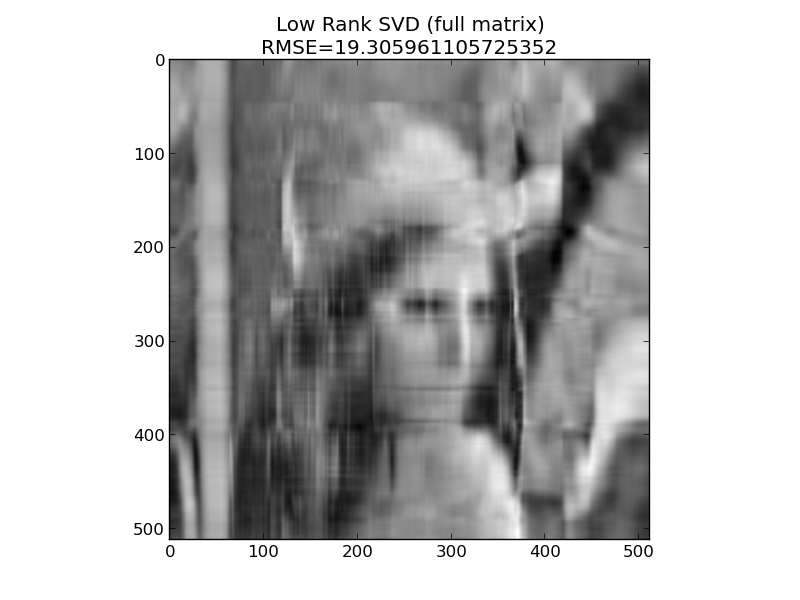
\includegraphics[width=0.45\textwidth]{fullsvd.png}
    \caption{Full matrix SVD}
    \label{fig:fullSVD}
\end{figure}
\begin{figure}[h!]
\centering
    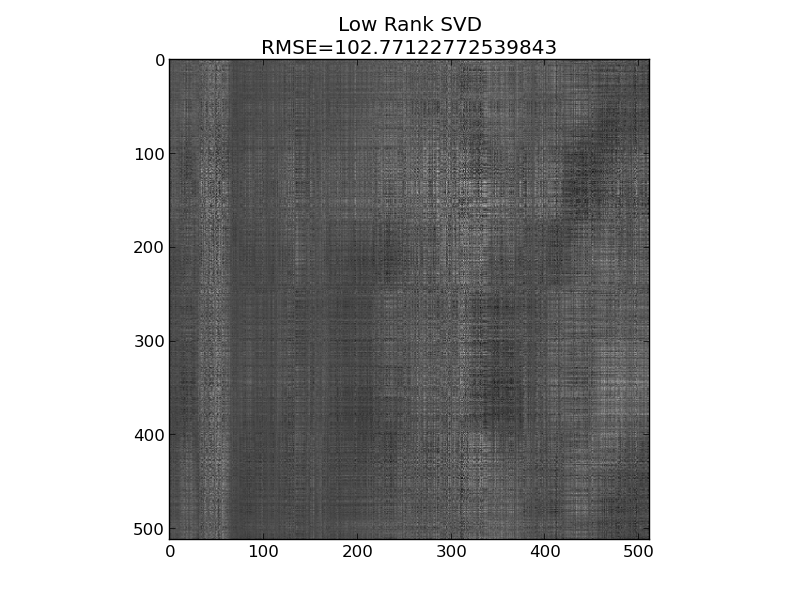
\includegraphics[width=0.45\textwidth]{sparsesvd.png}
    \caption{Sparse matrix SVD}
    \label{fig:sparseSVD}
\end{figure}

\section{PMF}

%\subsection{Notes}
%\begin{equation}
%    x_q = x_n + e_n
%\end{equation}
%\begin{thebibliography}{1}
%
%\begin{figure}[h!]
%\centering
%  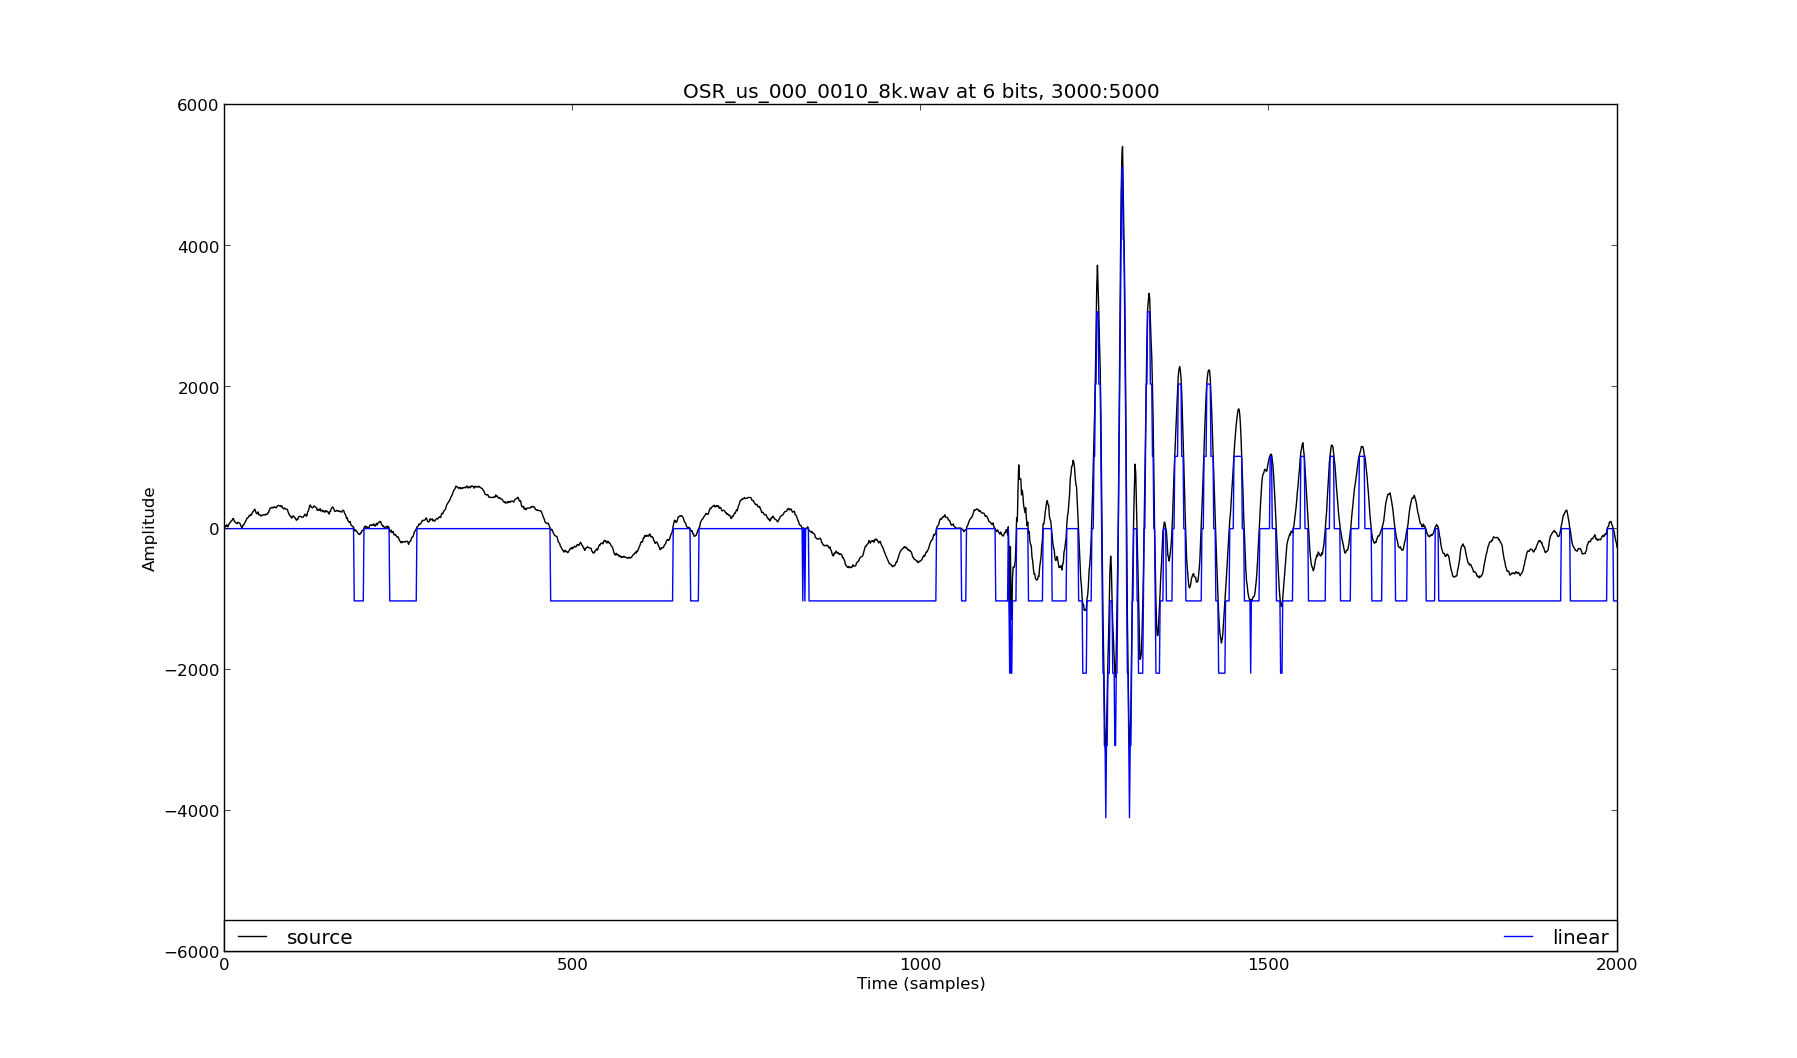
\includegraphics[width=0.45\textwidth]{linear_6bit.png}
%\caption{Linear quantization, $B = 6$}
%\label{fig:linear}
%\end{figure}
%\ref{fig:linear}

\begin{thebibliography}{1}
\bibitem{RMSE}
Unknown Author, \emph{Root Mean Square Error}. Taken from http://www.ctec.ufal.br/professor/crfj/Graduacao/MSH/Model\%20evaluation\%20methods.doc,
on May 10, 2013.
\bibitem{SVDTutorial}
K. Baker, \emph{Singular Value Decomposition Tutorial}. Taken from 
http://www.ling.ohio-state.edu/~kbaker/pubs/Singular\_Value\_Decomposition\_Tutorial.pdf, on May 9, 2013.
\bibitem{SVDIntuition}
Unknown Author, \emph{The Singular Value Decomposition in Symmetric Orthogonalization and Data Compression}.
Taken from http://www.wou.edu/~beavers/Talks/Willamette1106.pdf, on May 10, 2013.
\bibitem{SCIPYsource}
SciPy community, \emph{Sparse Eigenvalue Problems with ARPACK}. 
Taken from http://docs.scipy.org/doc/scipy/reference/tutorial/arpack.html, on May 10, 2013.
\bibitem{ARPACKsource}
R. Lehoucq, K. Maschhoff, D. Sorensen, C. Yang, \emph{ARPACK Documentation}. Taken from http://www.caam.rice.edu/software/ARPACK/, on May 10, 2013.
\end{thebibliography}

% You can push biographies down or up by placing
% a \vfill before or after them. The appropriate
% use of \vfill depends on what kind of text is
% on the last page and whether or not the columns
% are being equalized.

%\vfill

% Can be used to pull up biographies so that the bottom of the last one
% is flush with the other column.
%\enlargethispage{-5in}

% that's all folks
\end{document}


